\documentclass[sigconf,nonacm]{acmart}

% AI4F '26 (3rd Workshop on LLMs and Generative AI for Finance), ACM ICAIF '26.
% Review is SINGLE-blind (ai4f.org, checked 2026-10-10): authors are named.
% No length limit; PDF; ACM sigconf recommended. Deadline Oct 12, 2026 AoE.
%
% v2 draft, rebuilt around the Oct 9 results. Supersedes main.tex (Oct 6), which
% still carries the retracted "truncation inflates the size effect" claim.
%
% Every number is a macro: numbers.tex (paper/make_numbers.py) and numbers_r9.tex
% (paper/make_numbers_r9.py). Nothing is hand-typed. The human rater check was
% dropped (Oct 12); it was never in the pre-registered plan, so this is not a deviation.

\settopmatter{printacmref=false}
\usepackage{booktabs}
\usepackage{graphicx}
\usepackage{xcolor}
\usepackage{tabularx}

% Generated by paper/make_numbers.py — DO NOT EDIT BY HAND.
% Regenerate with: make numbers
\providecommand{\todo}[1]{\textcolor{red}{\textbf{[TODO: #1]}}}

% --- sample and extraction ---
\newcommand{\NFilings}{59}
\newcommand{\NFirms}{30}
\newcommand{\NWindows}{667}
\newcommand{\NCalls}{2,001}
\newcommand{\NWindowsMDA}{363}
\newcommand{\NCallsMDA}{1,089}
\newcommand{\NFilingsWithRisk}{49}
\newcommand{\NFilingsNoRisk}{10}
\newcommand{\MdaWindowsMedianLarge}{6.5}
\newcommand{\MdaWindowsMedianMid}{6.5}
\newcommand{\MdaWindowsMedianSmall}{4.0}
\newcommand{\MdaWordsMin}{2,675}
\newcommand{\MdaWordsMax}{30,340}

% --- the coverage confound (retired 2,000-word cap) ---
\newcommand{\CoverageRho}{-0.415}
\newcommand{\CoverageP}{0.001}
\newcommand{\CoverageN}{59}
\newcommand{\NTruncated}{59}
\newcommand{\FracReadLarge}{12.9}
\newcommand{\SectionWordsLarge}{15,488}
\newcommand{\FracReadMid}{17.0}
\newcommand{\SectionWordsMid}{11,750}
\newcommand{\FracReadSmall}{27.5}
\newcommand{\SectionWordsSmall}{7,285}

% --- primary result (MD&A embedding disagreement, firm level) ---
\newcommand{\TierMeanLarge}{0.3202}
\newcommand{\TierSDLarge}{0.0341}
\newcommand{\TierMeanMid}{0.3355}
\newcommand{\TierSDMid}{0.0312}
\newcommand{\TierMeanSmall}{0.3352}
\newcommand{\TierSDSmall}{0.0218}
\newcommand{\PrimaryGradient}{0.0150}
\newcommand{\PrimaryJT}{169.0}
\newcommand{\PrimaryJTz}{0.722}
\newcommand{\PrimaryJTp}{0.235}
\newcommand{\PrimaryPermP}{0.242}
\newcommand{\PrimaryMonotone}{no}

% --- window-count battery ---
\newcommand{\WThreeShare}{0.885}
\newcommand{\WThreePassed}{no}
\newcommand{\GateBatteryPassed}{no}
\newcommand{\WSixPercentile}{91.4}
\newcommand{\WSixP}{0.086}

% --- W5 mixed model ---
\newcommand{\WFiveSpec}{firm\_only}
\newcommand{\WFiveSmallCoef}{0.0142}
\newcommand{\WFiveSmallCIlo}{-0.0126}
\newcommand{\WFiveSmallCIhi}{0.0411}
\newcommand{\WFiveSmallP}{0.299}
\newcommand{\ICCFilingNonConverged}{0.231}
\newcommand{\ICCFirm}{0.077}
\newcommand{\VarWithinFiling}{0.783}
\newcommand{\VarWithinFilingPct}{78.3}
\newcommand{\WFiveCriterionMet}{no}

% --- R1 reliability ---
\newcommand{\SplitHalfR}{0.136}
\newcommand{\SplitHalfSB}{0.239}
\newcommand{\TestRetestR}{0.276}
\newcommand{\TestRetestP}{0.147}

% --- numeric measure / retirement rule ---
\newcommand{\NumericLengthRho}{0.046}
\newcommand{\NumericLengthP}{0.727}
\newcommand{\NumericLengthN}{59}
\newcommand{\NumericRetired}{no}

% --- S2 at-scale audit ---
\newcommand{\ScaleNUsable}{785}
\newcommand{\ScaleSuccessPct}{98.1}
\newcommand{\ScaleElasticity}{0.0527}
\newcommand{\ScaleRho}{0.161}
\newcommand{\ScaleP}{<0.001}
\newcommand{\ScaleTruncTwoK}{99.1}
\newcommand{\ScaleMedianReadTwoK}{9.5}
\newcommand{\ScaleTruncThirtyTwoK}{39.7}

% --- E1/E2 noise floor (partial: interrupted by rate limiting) ---
\newcommand{\NoiseN}{27}
\newcommand{\NoiseRatio}{1.64}
\newcommand{\NoiseLensEffect}{0.1395}
\newcommand{\NoiseInter}{0.3454}
\newcommand{\NoiseIntra}{0.2142}
\newcommand{\NoiseNeutral}{0.2059}

% --- S1b truncation replication (the headline) ---
\newcommand{\TruncLarge}{0.3350}
\newcommand{\TruncMid}{0.3706}
\newcommand{\TruncSmall}{0.3921}
\newcommand{\TruncGradient}{0.0571}
\newcommand{\TruncP}{0.029}
\newcommand{\TruncMonotone}{yes}
\newcommand{\CompLarge}{0.3202}
\newcommand{\CompMid}{0.3355}
\newcommand{\CompSmall}{0.3352}
\newcommand{\CompGradient}{0.0150}
\newcommand{\CompP}{0.235}
\newcommand{\CompMonotone}{no}
\newcommand{\PairedDelta}{0.0356}
\newcommand{\PairedDeltaLo}{0.0172}
\newcommand{\PairedDeltaHi}{0.0540}
\newcommand{\PairedDeltaN}{30}

% --- E4 content placebo / E6 familiarity ---
\newcommand{\PlacReal}{0.3199}
\newcommand{\PlacShuffled}{0.3379}
\newcommand{\PlacBoilerplate}{0.3587}
\newcommand{\PlacAnonymised}{0.3127}
\newcommand{\PlacDiffShuffled}{-0.0173}
\newcommand{\PlacDiffShuffledLo}{-0.0470}
\newcommand{\PlacDiffShuffledHi}{0.0142}
\newcommand{\PlacDiffBoilerplate}{-0.0389}
\newcommand{\PlacDiffBoilerplateLo}{-0.0654}
\newcommand{\PlacDiffBoilerplateHi}{-0.0110}
\newcommand{\PlacN}{36}

% --- F2 informativeness ---
\newcommand{\NumDensityRho}{-0.260}
\newcommand{\NumDensityP}{<0.001}
\newcommand{\DisagMDA}{0.3291}
\newcommand{\DisagRisk}{0.3510}

% --- E7 cross-model ---

% --- provenance ---
\newcommand{\GitHash}{6cc128b}
\newcommand{\PlanHashFirst}{fec1eb2}
\newcommand{\PlanHashUsed}{c22f5dd}
\newcommand{\PlanAmendments}{2}
\newcommand{\ModelName}{openai/gpt-oss-20b}
\newcommand{\ChunkWords}{1,200}


% Generated by paper/make_numbers_r9.py -- DO NOT EDIT BY HAND.
\providecommand{\todo}[1]{\textcolor{red}{\textbf{[TODO: #1]}}}
% --- S1c decomposition (same-backend arms) ---
\newcommand{\DecTruncSingleGrad}{+0.0295}
\newcommand{\DecTruncSingleP}{0.191}
\newcommand{\DecCompSingleGrad}{+0.0435}
\newcommand{\DecCompSingleP}{0.074}
\newcommand{\DecCoverageEffect}{-0.0139}
\newcommand{\DecCoveragePaired}{-0.0252}
\newcommand{\DecCoveragePairedLo}{-0.0534}
\newcommand{\DecCoveragePairedHi}{+0.0027}
\newcommand{\DecUnitEffect}{+0.0285}
\newcommand{\DecAggEffect}{+0.0002}
\newcommand{\DecOneWindowGrad}{+0.0152}
\newcommand{\DecOneWindowLo}{-0.0239}
\newcommand{\DecOneWindowHi}{+0.0563}
\newcommand{\DecSOneAkTwoGrad}{+0.0204}
% --- S3 classical measures ---
\newcommand{\FogDistLarge}{+1.86}
\newcommand{\FogDistLargeLo}{+0.21}
\newcommand{\FogDistLargeHi}{+3.79}
\newcommand{\FogDistMid}{-0.43}
\newcommand{\FogDistSmall}{+0.38}
\newcommand{\FogGradShift}{-1.49}
\newcommand{\FogGradTrunc}{-1.41}
\newcommand{\FogGradComp}{+0.08}
\newcommand{\UncDistLarge}{+0.28}
\newcommand{\UncDistLargeLo}{+0.02}
\newcommand{\UncDistLargeHi}{+0.56}
\newcommand{\NegPTrunc}{0.092}
\newcommand{\NegPComp}{0.395}
% --- S2 scale table ---
\newcommand{\ScFiveTwelveMed}{1.8}
\newcommand{\ScFiveTwelveBot}{2.6}
\newcommand{\ScFiveTwelveTop}{1.8}
\newcommand{\ScFiveTwelveTrunc}{100.0}
\newcommand{\ScTwoKMed}{9.5}
\newcommand{\ScTwoKBot}{13.4}
\newcommand{\ScTwoKTop}{9.3}
\newcommand{\ScTwoKTrunc}{99.1}
\newcommand{\ScFourKMed}{14.6}
\newcommand{\ScFourKBot}{20.5}
\newcommand{\ScFourKTop}{14.3}
\newcommand{\ScFourKTrunc}{97.7}
\newcommand{\ScEightKMed}{29.3}
\newcommand{\ScEightKBot}{41.1}
\newcommand{\ScEightKTop}{28.5}
\newcommand{\ScEightKTrunc}{93.8}
\newcommand{\ScThirtyTwoKMed}{100.0}
\newcommand{\ScThirtyTwoKBot}{100.0}
\newcommand{\ScThirtyTwoKTop}{100.0}
\newcommand{\ScThirtyTwoKTrunc}{39.7}
\newcommand{\ScSpotN}{20}
\newcommand{\ScSpotPass}{20}
\newcommand{\ScNAttempted}{800}
% --- E4 / E4b / E6 ---
\newcommand{\PlacRealLo}{0.2966}
\newcommand{\PlacRealHi}{0.3435}
\newcommand{\PlacShufLo}{0.3125}
\newcommand{\PlacShufHi}{0.3632}
\newcommand{\PlacBoilLo}{0.3408}
\newcommand{\PlacBoilHi}{0.3762}
\newcommand{\AnonDiff}{+0.0071}
\newcommand{\AnonDiffLo}{-0.0153}
\newcommand{\AnonDiffHi}{+0.0297}
\newcommand{\AnonLarge}{-0.0238}
\newcommand{\AnonMid}{+0.0412}
\newcommand{\AnonSmall}{+0.0099}
\newcommand{\BpN}{10}
\newcommand{\BpMean}{0.3874}
\newcommand{\BpLo}{0.3305}
\newcommand{\BpHi}{0.4510}
\newcommand{\BpSD}{0.1029}
\newcommand{\BpMin}{0.2522}
\newcommand{\BpMax}{0.6156}
\newcommand{\BpRealMean}{0.3291}
\newcommand{\BpRealLo}{0.3215}
\newcommand{\BpRealHi}{0.3370}
\newcommand{\BpRealN}{362}
\newcommand{\BpDiff}{+0.0583}
% --- E7 cross-model ---
\newcommand{\XmN}{50}
\newcommand{\XmReal}{0.2797}
\newcommand{\XmRealLo}{0.2582}
\newcommand{\XmRealHi}{0.3019}
\newcommand{\XmShuf}{0.2967}
\newcommand{\XmShufLo}{0.2756}
\newcommand{\XmShufHi}{0.3189}
\newcommand{\XmBoil}{0.3036}
\newcommand{\XmBoilLo}{0.2898}
\newcommand{\XmBoilHi}{0.3173}
\newcommand{\XmDiffShuf}{-0.0170}
\newcommand{\XmDiffShufLo}{-0.0398}
\newcommand{\XmDiffShufHi}{+0.0064}
\newcommand{\XmDiffBoil}{-0.0238}
\newcommand{\XmDiffBoilLo}{-0.0467}
\newcommand{\XmDiffBoilHi}{-0.0002}
\newcommand{\XmModel}{\texttt{meta-llama/llama-3.3-70b-instruct}}
\newcommand{\XmBackend}{Novita}
% --- secondary family (Holm, two-sided) ---
\newcommand{\SecNumGrad}{-0.0544}
\newcommand{\SecNumP}{0.119}
\newcommand{\SecNumHolm}{0.357}
\newcommand{\SecNumLarge}{0.5978}
\newcommand{\SecNumMid}{0.5981}
\newcommand{\SecNumSmall}{0.5434}
\newcommand{\SecRiskGrad}{-0.0114}
\newcommand{\SecRiskP}{0.833}
\newcommand{\SecRiskHolm}{1.000}
\newcommand{\SecRiskFirms}{28}
\newcommand{\SecRiskFilings}{49}
\newcommand{\SecSDGrad}{-0.0046}
\newcommand{\SecSDP}{0.594}
\newcommand{\SecSDHolm}{1.000}
% --- continuous size ---
\newcommand{\ContRho}{-0.295}
\newcommand{\ContP}{0.114}
\newcommand{\ContLo}{-0.601}
\newcommand{\ContHi}{+0.109}
\newcommand{\ContSlope}{-0.0067}
\newcommand{\ContNumRho}{+0.235}
\newcommand{\ContNumP}{0.211}
\newcommand{\ContRiskRho}{+0.020}
\newcommand{\ContRiskP}{0.919}
\newcommand{\ContTierRho}{0.910}
\newcommand{\ContFloatMinM}{27.6}
\newcommand{\ContFloatMaxT}{3.6}
% --- HAYN sensitivity ---
\newcommand{\HaynGrad}{+0.0172}
\newcommand{\HaynP}{0.179}
\newcommand{\HaynPermP}{0.185}
\newcommand{\HaynN}{29}
% --- E1/E2 CIs and tier n ---
\newcommand{\NoiseRatioLo}{1.52}
\newcommand{\NoiseRatioHi}{1.75}
\newcommand{\NoiseLensLo}{0.104}
\newcommand{\NoiseLensHi}{0.175}
\newcommand{\NoiseNLarge}{11}
\newcommand{\NoiseNMid}{8}
\newcommand{\NoiseNSmall}{8}
% --- E3 ---
\newcommand{\EncRhoMpnet}{0.755}
\newcommand{\EncRhoBge}{0.713}
\newcommand{\EncPMin}{0.18}
\newcommand{\EncPMax}{0.38}
% --- D1 ---
\newcommand{\DOneLen}{-0.148}
\newcommand{\DOneFog}{-0.007}
\newcommand{\DOneNeg}{-0.083}
\newcommand{\DOneUnc}{-0.032}
\newcommand{\DOneLit}{+0.072}
\newcommand{\DOneTTR}{0.212}
\newcommand{\DOneTTRp}{0.107}
\newcommand{\DOneRsq}{0.148}
% --- R1 numeric + extrapolation ---
\newcommand{\SplitHalfSBNumeric}{0.520}
\newcommand{\SplitHalfN}{48}
\newcommand{\TestRetestN}{29}
\newcommand{\RelWindowsSeventy}{37}
\newcommand{\RelWordsSeventy}{44,550}
% --- F1/F2 ---
\newcommand{\InfTTRRho}{+0.213}
\newcommand{\InfWordLenRho}{+0.214}
\newcommand{\InfWordCountRho}{+0.071}
\newcommand{\InfWordCountP}{0.068}
\newcommand{\PosRho}{-0.091}
\newcommand{\PosP}{0.020}
\newcommand{\TopicLit}{+0.0161}
\newcommand{\TopicGuid}{+0.0121}
\newcommand{\TopicAcct}{-0.0088}
\newcommand{\CaseLowDisag}{0.1525}
\newcommand{\CaseLowDensity}{0.037}
\newcommand{\CaseHighDisag}{0.5550}
\newcommand{\CaseHighDensity}{0.002}
% --- battery values the v1 draft hand-typed ---
\newcommand{\WOneRho}{0.372}
\newcommand{\WOneP}{0.004}
\newcommand{\WTwoCEM}{+0.0231}
\newcommand{\WFourFirstTwo}{+0.0204}
\newcommand{\WFourExclFirst}{+0.0107}
\newcommand{\WSevenExact}{+0.0101}
\newcommand{\WSixNullPNinetyFive}{0.0218}
\newcommand{\WSixNullMean}{-0.0000}
\newcommand{\WSixNullSD}{0.0110}
\newcommand{\WinWordsMin}{403}
\newcommand{\WinWordsMax}{1,577}
\newcommand{\PermGradP}{0.132}
\newcommand{\PermGradNullSD}{0.0132}
\newcommand{\WThreeKFourShare}{0.789}
% --- W5 OLS-cluster ---
\newcommand{\WFiveICCFilingNC}{0.231}



\begin{document}

\title{Disagreement About Nothing: A Pre-Registered Stress Test of a
Persona-Ensemble Measure of 10-K Complexity}

% TODO(before submission): authorship and order have NOT been agreed with
% Prof. Pukthuanthong. The OpenReview author list cannot be changed after
% submission. Confirm with her before uploading.
\author{Aryan Chhabra}
\affiliation{%
  \institution{University of Missouri}
  \city{Columbia}\state{Missouri}\country{USA}}
\email{aryanchhabra6996@gmail.com}

\author{Kuntara Pukthuanthong}
\affiliation{%
  \institution{University of Missouri}
  \city{Columbia}\state{Missouri}\country{USA}}

\begin{abstract}
LLM pipelines that score financial filings make harness decisions that are rarely
reported: how much of the filing to read, in what unit, and on which serving backend.
We stress-test one such pipeline under a plan registered before any filing was scored.
The measure is persona disagreement. One fixed model (\texttt{gpt-oss-20b}, a single
\texttt{bf16} backend) reads every \ChunkWords-word window of a filing's complete MD\&A
through three analytical lenses, and the embedding distance between their rationales
is taken as an index of interpretive complexity. On \NFilings{} filings from \NFirms{}
firms the measure passes the checks such measures usually report: it clears a
same-prompt noise floor (\NoiseRatio$\times$), is stable across three sentence
encoders, and is uncorrelated with length, readability and dictionary tone. It fails
the check that matters. Replacing real MD\&A with content-free safe-harbor boilerplate
\emph{raises} disagreement, on two model families; disagreement falls as a window
carries more figures; and filing-level split-half reliability is \SplitHalfSB. The
pre-registered size test is null ($p=\PrimaryJTp$). On the harness side, a
2,000-word budget truncates \ScaleTruncTwoK\% of \ScaleNUsable{} 10-Ks and moves Fog
and Loughran--McDonald uncertainty for large firms only. For the LLM measure, reading
those 2,000 words as one block yields a significant size effect ($p=\TruncP$) that
disappears under windowing, weakens to $p=\DecTruncSingleP$ on a second \texttt{bf16}
backend serving the same weights, and cannot be attributed to coverage. We close with a short reporting
checklist for LLM-derived text measures in finance.
\end{abstract}

\keywords{large language models, financial disclosure, 10-K, evaluation, measurement
validity, pre-registration, harness engineering}

\maketitle

% =====================================================================
\section{Introduction}

A growing body of work asks language models to read corporate disclosure and return a
number: a sentiment score, a forecast, a complexity rating~\cite{kmn2023, ll2023}.
Before any of that happens, someone has to decide how the filing reaches the model.
Annual reports run to tens of thousands of words, so the text is cut to a budget, or
split into chunks and the chunk scores averaged, and the calls are routed to whatever
endpoint serves the model. These choices are usually reported in a sentence. They are
also exactly the kind of choice a workshop on harness engineering and evaluation should
care about, because they sit between the data and the conclusion and nobody checks them.

We built a measure, wrote down in advance how it would be tested, and then tested it
until it broke. The measure asks whether a filing pulls different analytical
perspectives apart. Three personas (a value investor, a disclosure-language analyst, a
fundamentals analyst) read the same text under one fixed model, and the distance
between their written rationales is the score. The hypothesis was the obvious one:
smaller, less-followed firms write filings that are harder to interpret, so their
filings should split the lenses further.

The paper makes three contributions.

\textbf{A validity failure that standard checks miss.} Persona disagreement clears a
noise floor, survives a change of encoder, is uncorrelated with length and tone, and
shows no familiarity effect. Each of those is a check papers in this area commonly
report. It still does not measure what it was built to measure: content-free
boilerplate produces \emph{more} disagreement than real MD\&A on two model families,
and disagreement is highest where a window offers nothing concrete to agree on. A
measure of this kind is responding to the absence of information, not to the difficulty
of interpreting it.

\textbf{Harness choices move the answer, but not the one we expected.} A fixed reading
budget makes coverage a function of firm size across \ScaleNUsable{} 10-Ks, and it
distorts two established textual measures for large firms only. For the LLM measure,
though, a careful decomposition shows coverage is not what matters. Reading the first
2,000 words as one block produces a significant, monotone size effect; reading the same
filings complete, in windows, does not. Neither coverage nor averaging accounts for the
gap, and the single-block result itself weakens sharply when the same weights are
served by a different \texttt{bf16} provider.

\textbf{A pre-registered null, reported with the diagnostics that explain it.} The
confirmatory size test, a pre-registered battery for window-count artifacts, a
Holm-corrected secondary family, a pre-specified exclusion, and an exploratory test on
continuous public float all fail to find the predicted gradient. Filing-level
reliability of \SplitHalfSB{} explains why: most of the variance lives between windows
of the same filing. We turn the lessons into a reporting checklist
(Section~\ref{sec:discussion}).

% =====================================================================
\section{Related Work}

\textbf{Complexity in disclosure.} Accounting research has measured the readability
and length of annual reports for decades and related them to earnings persistence,
information processing and obfuscation~\cite{li2008, bgt2018}. Loughran and McDonald
showed that general-purpose word lists and readability formulas misfire on financial
text and built finance-specific alternatives~\cite{lm2011, lm2014, lm2016}. Those
measures are the natural benchmarks for any new complexity score, and we use them as
such.

\textbf{Disagreement.} Divergence of opinion has long been treated as economically
meaningful~\cite{miller1977, dms2002}. Our measure is a mechanical cousin: dispersion
among prompted lenses applied by one model to one text, rather than dispersion among
analysts.

\textbf{LLMs on financial text.} Recent work applies language models to disclosure
summarization and return prediction~\cite{kmn2023, ll2023}, and a parallel strand warns
that models may have memorized the firms and periods under study~\cite{glasserman2023}.
In the ML literature, disagreement among sampled outputs is used as an uncertainty
signal~\cite{wang2023sc, kuhn2023semantic}; our placebo result is a caution about
reading such disagreement as a property of the input. Long inputs degrade
retrieval~\cite{liu2024lost}, and nominally deterministic LLM settings still vary
across runs~\cite{atil2024}; both bear directly on the harness choices we test.

% =====================================================================
\section{Data and Harness}
\label{sec:data}

\subsection{Sample}
\NFirms{} firms in three size tiers of ten, each contributing its most recent 10-K and
10-Q filed after July 1, 2024, for \NFilings{} filings (one firm was acquired and delisted
before filing a 10-K and contributes a 10-Q only). The model card for \texttt{gpt-oss-20b}
states a June 2024 knowledge cutoff~\cite{gptoss2025}, so every filing postdates the
model's training data. The sample is frozen in a manifest pinned by ticker, form and
date, and the whole analysis reproduces offline from cached filings and cached model
output. Code, cached model output, the analysis plan and the deviation log are at
\url{https://github.com/aryanch09/interpretive-complexity-pilot}.

\subsection{Complete-section extraction}
MD\&A and Risk Factors are extracted whole, with no word cap. This turned out to be the
hardest engineering in the project, and the failures it uncovered are silent under a
cap. One large bank's ``MD\&A'' initially ran to 107{,}257 words because the span
continued into the financial statements. A standard HTML-cleaning step that drops
small tables deleted item headings that some filers render as one-cell tables, which
removed one large-cap filing's entire Risk Factors section and silently truncated
three large-cap MD\&As. Both errors ran in the same direction as the confound studied
below: they shortened \emph{large-cap} text. After the fixes, MD\&A runs from
\MdaWordsMin{} to \MdaWordsMax{} words, every filing yields a usable MD\&A, and the
\NFilingsNoRisk{} filings without Risk Factors are 10-Qs that incorporate the 10-K's
risk factors by reference, each verified by hand.

\subsection{Windows, personas and serving}
Each section is split into non-overlapping \ChunkWords-word windows (a remainder under
400 words merges into the previous window). Every window is read by three persona
prompts under one model, \ModelName, at temperature 0.3, with no interaction between
calls. Each persona returns a 0--100 score, a confidence, a 3--5 sentence rationale and
key factors (Appendix~\ref{app:prompts}). This is a prompt ensemble: the model is held
fixed and only the analytical lens varies. The run covers \NWindows{} windows and
\NCalls{} calls; \NWindowsMDA{} of the windows are MD\&A, and \NFirms{} of \NFirms{} firms and
all \NFilings{} filings survive the rule that drops any window in which a persona
failed.

All calls go to a single provider at \texttt{bf16}, with routing fallbacks disabled.
This is a methodological requirement rather than an optimization. The router we used
serves this model from many endpoints at fp4, fp8, \texttt{bf16} and undeclared
precision; default load-balancing would mix them, and some of the measured disagreement
would then be a quantization artifact. The pipeline logs which backend served each call
and fails the run if more than one did.

\subsection{Measures and pre-registration}
Window-level disagreement is the mean pairwise cosine distance between the three
rationales' sentence embeddings~\cite{sbert2019}, computed with \texttt{all-MiniLM-L6-v2}
(primary), and the standard deviation of the three scores (secondary). A filing's value is the
unweighted mean over its MD\&A windows; a firm's is the mean over its filings. The
firm is the unit for every confirmatory test.

The analysis plan was committed before any filing was scored (commit
\texttt{\PlanHashFirst}, amended \PlanAmendments{} times before scoring, final
\texttt{\PlanHashUsed}). It fixed the primary outcome (MD\&A only), one confirmatory
test (a one-sided Jonckheere--Terpstra trend test~\cite{jonckheere1954} on firm means,
with a label-permutation check), a battery of window-count tests with pass criteria, a
two-sided secondary family under Holm correction~\cite{holm1979}, and a definition of a
null. Every deviation is logged (Appendix~\ref{app:deviations}), including one
correction made after a number had been computed.

% =====================================================================
\section{What the Harness Does to the Answer}
\label{sec:harness}

\subsection{Coverage is a function of firm size}

\begin{figure*}[t]
  \centering
  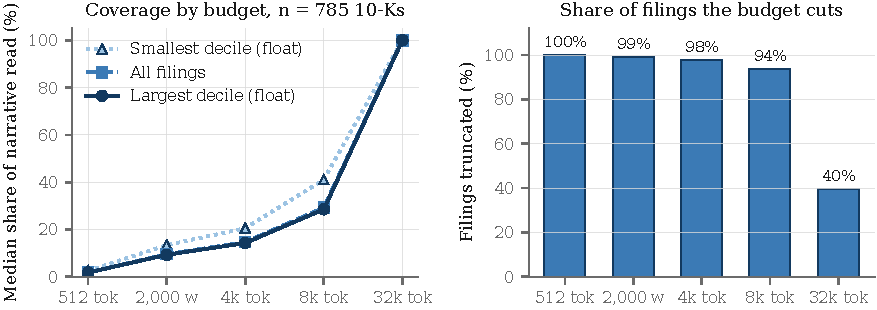
\includegraphics[width=0.86\textwidth]{figures/fig_r9_scale.pdf}
  \caption{Fixed reading budgets across \ScaleNUsable{} 10-Ks, with firm size
  taken from each filer's own reported public float. Left: median share of the
  MD\&A plus Risk Factors narrative that fits in the budget, for the smallest and
  largest float deciles. Right: share of filings the budget truncates. Token budgets
  converted at 0.75 words per token.}
  \label{fig:scale}
\end{figure*}

We measured complete narrative length for \ScaleNUsable{} 10-K filings drawn across
public-float deciles, with zero model calls, taking size from
\texttt{dei:EntityPublicFloat} on each filer's own cover page. Extraction succeeded on
\ScaleSuccessPct\% of \ScNAttempted{} attempts, and a seeded random spot check of
\ScSpotN{} extractions found \ScSpotPass{} that began at a real MD\&A heading and ended
before the financial statements. Narrative length rises with float (Spearman
$\rho=\ScaleRho$, $p\ScaleP$), so a fixed budget reads a smaller share of a larger
firm's filing. At 2,000 words the median filing in the smallest float decile is read at
\ScTwoKBot\% and in the largest at \ScTwoKTop\% (Figure~\ref{fig:scale}).

The gradient is real but modest; the elasticity of length on float is
\ScaleElasticity. The blunter fact is the level. A 2,000-word budget truncates
\ScTwoKTrunc\% of filings, an 8k-token budget \ScEightKTrunc\%, and even 32k tokens cuts
\ScThirtyTwoKTrunc\%. In our own stratified sample the retired 2,000-word cap read the
median large-cap filing at \FracReadLarge\% and the median small-cap at
\FracReadSmall\% ($\rho=\CoverageRho$ between size rank and share read,
$p=\CoverageP$).

\textbf{Established measures inherit the confound.} To check that this matters outside
our own measure, we computed Fog~\cite{gunning1952} and Loughran--McDonald
category shares~\cite{lm2011} on each firm's MD\&A twice, complete and truncated at
2,000 words, with identical code. Truncation raised large-cap Fog by \FogDistLarge{}
points [\FogDistLargeLo, \FogDistLargeHi] and large-cap uncertainty share by
\UncDistLarge{} percentage points [\UncDistLargeLo, \UncDistLargeHi], while mid- and
small-cap Fog moved by \FogDistMid{} and \FogDistSmall. That is the coverage mechanism:
large-cap filings are the ones a cap cuts hardest. The small-minus-large Fog gradient
moves from \FogGradComp{} complete to \FogGradTrunc{} truncated. With ten firms per tier
most intervals are wide, so we present this as directional evidence that the confound is
not specific to language models.

\subsection{For the LLM measure, the scoring unit matters, not coverage}

\begin{table}[t]
  \caption{The size gradient (small minus large, firm-level means of MD\&A persona
  disagreement) under different harness choices. Backend A is the provider used for
  the main run; backend B is a second \texttt{bf16} provider serving the same weights.
  $p$ is the one-sided Jonckheere--Terpstra test.}
  \label{tab:harness}
  \small
  \begin{tabular}{@{}llrr@{}}
    \toprule
    Text read & Unit, backend & Gradient & $p$ \\
    \midrule
    Complete (pre-registered) & windows, A & \PrimaryGradient & \PrimaryJTp \\
    Complete & 1 random window, A & \DecOneWindowGrad & -- \\
    First 2,000 w & one read, A & \TruncGradient & \TruncP \\
    First 2,000 w & one read, B & \DecTruncSingleGrad & \DecTruncSingleP \\
    Complete & one read, B & \DecCompSingleGrad & \DecCompSingleP \\
    \midrule
    \multicolumn{2}{@{}l}{Coverage effect (same unit, same backend)} & \DecCoverageEffect & \\
    \multicolumn{4}{@{}l}{\quad paired per-firm: \DecCoveragePaired{}, 95\% CI [\DecCoveragePairedLo, \DecCoveragePairedHi]} \\
    \multicolumn{2}{@{}l}{Averaging effect (all vs.\ one window)} & \DecAggEffect & \\
    \multicolumn{2}{@{}l}{Unit effect (one read vs.\ windows)$^\dagger$} & \DecUnitEffect & \\
    \bottomrule
  \end{tabular}

  \raggedright\footnotesize $^\dagger$Confounded with backend; indicative only.
\end{table}

The retired version of this pipeline read each filing's first 2,000 words of MD\&A as
a single unit. Re-scoring exactly that, with the same model, filings and personas,
gives a monotone size gradient of \TruncGradient{} ($p=\TruncP$), against
\PrimaryGradient{} ($p=\PrimaryJTp$) for the complete, windowed run; the paired
per-firm difference is \PairedDelta{} [\PairedDeltaLo, \PairedDeltaHi]. An earlier
version of this work read that as truncation manufacturing a false positive. The
decomposition in Table~\ref{tab:harness} does not support that reading.

The two arms differ in three ways at once: how much text is read, whether it is read in
one block or in windows, and how many scores are averaged. Averaging can be isolated
for free. Taking one random window per filing instead of the mean of all of them leaves
the gradient at \DecOneWindowGrad, an averaging effect of \DecAggEffect, as it should
be, since averaging changes the variance of a filing mean and not its expectation.
Coverage needs one more arm: the complete MD\&A scored as a single unit. Scoring both
single-unit arms on the same backend, the coverage effect on the gradient is
\DecCoverageEffect, paired \DecCoveragePaired{} [\DecCoveragePairedLo,
\DecCoveragePairedHi]. That is the opposite sign to the claim, and the interval spans
zero. What remains is the scoring unit, about \DecUnitEffect, and that comparison is
confounded with backend.

The backend matters on its own account. The truncated single-read arm was run on both
providers, at the same precision and with the same weights and prompts; the gradient is
\TruncGradient{} ($p=\TruncP$) on one and \DecTruncSingleGrad{} ($p=\DecTruncSingleP$)
on the other. We do not think this means either provider is wrong. It means a
cross-sectional result at $n=\NFirms$ can sit within the variation introduced by
serving infrastructure~\cite{atil2024}, which is a reason to pin and report the
backend, and to treat any single significant contrast from one serving configuration
with suspicion.

Two cautions apply to the decomposition. A single read of a complete MD\&A (up to
\MdaWordsMax{} words) is the design we originally rejected because long-context
degradation is worst for the longest sections~\cite{liu2024lost}, which belong to the
largest firms, so that arm carries a size-correlated bias of its own; the decomposition
bounds the effects rather than identifying them. And because the measure itself turns
out to be invalid (Section~\ref{sec:validity}), what the scoring unit is changing is not
interpretive complexity. The defensible harness finding is narrow: for this class of
LLM measure, how a filing is chunked and on what it is served moved the cross-sectional
answer more than how much of it was read.

% =====================================================================
\section{Is Persona Disagreement a Measure?}
\label{sec:validity}

\begin{table}[t]
  \caption{Validity checks on window-level MD\&A persona disagreement. ``Pass'' means
  the result is what a valid measure of interpretive complexity would show.}
  \label{tab:validity}
  \footnotesize
  \begin{tabularx}{\columnwidth}{@{}Xll@{}}
    \toprule
    Check & Result & Verdict \\
    \midrule
    Noise floor: 3 lenses vs.\ 1 lens $\times$3 ($n=\NoiseN$) & ratio \NoiseRatio{} [\NoiseRatioLo, \NoiseRatioHi] & pass \\
    Persona-free baseline (neutral $\times$3) & $+$\NoiseLensEffect{} [\NoiseLensLo, \NoiseLensHi] & pass \\
    Encoder swap (2 alternatives), window $\rho$ & \EncRhoBge, \EncRhoMpnet & pass \\
    Length, Fog, L--M tone, TTR & all $|\rho|\le\DOneTTR$, n.s. & pass \\
    Anonymization (firm identity removed) & \AnonDiff{} [\AnonDiffLo, \AnonDiffHi] & pass \\
    \midrule
    Real $-$ sentence-shuffled, gpt-oss & \PlacDiffShuffled{} [\PlacDiffShuffledLo, \PlacDiffShuffledHi] & \textbf{fail} \\
    Real $-$ boilerplate, gpt-oss & \PlacDiffBoilerplate{} [\PlacDiffBoilerplateLo, \PlacDiffBoilerplateHi] & \textbf{fail} \\
    Real $-$ boilerplate, Llama-3.3-70B & \XmDiffBoil{} [\XmDiffBoilLo, \XmDiffBoilHi] & \textbf{fail} \\
    Figures per word vs.\ disagreement & $\rho=\NumDensityRho$ & \textbf{fail} \\
    Filing split-half (Spearman--Brown) & \SplitHalfSB & \textbf{fail} \\
    Same firm, 10-K vs.\ 10-Q & $r=\TestRetestR$ ($p=\TestRetestP$) & \textbf{fail} \\
    \bottomrule
  \end{tabularx}
\end{table}

Table~\ref{tab:validity} collects the checks. The top block is what such measures are
usually validated with, and our measure passes all of it.

\textbf{What it passes.} Running one persona three times on the same window gives a
noise floor; three different lenses disagree \NoiseRatio$\times$ as much, and three
copies of a neutral analyst prompt sit at the floor, so the lens does work the sampler
does not ($n=\NoiseN$ windows, \NoiseNLarge/\NoiseNMid/\NoiseNSmall{} by tier; the
planned subset was cut short by rate limiting). Re-encoding the cached rationales with
\texttt{all-mpnet-base-v2} and \texttt{bge-small-en-v1.5} gives window-level rank
correlations of \EncRhoMpnet{} and \EncRhoBge{}, and all three encoders agree there is
no size effect ($p=\EncPMin$ to \EncPMax). Filing-level disagreement is uncorrelated
with log length ($\rho=\DOneLen$), Fog (\DOneFog), and Loughran--McDonald negative
(\DOneNeg), uncertainty (\DOneUnc) and litigious (\DOneLit) shares; the largest
correlation, with type-token ratio, is \DOneTTR{} ($p=\DOneTTRp$). Stripping firm
names and tickers changes nothing (\AnonDiff), and no tier's anonymization delta clears
zero, so the shared model's familiarity with large firms is not suppressing their
disagreement.

We note that the first two checks are weaker than they look. Prompts that ask for
different things will produce text that embeds differently, so beating a noise floor
shows the lenses are distinct, not that their distance tracks anything about the filing.

\textbf{What it fails.} The bottom block asks the question that does bear on the
construct: does disagreement respond to the content of the filing?

\begin{figure}[t]
  \centering
  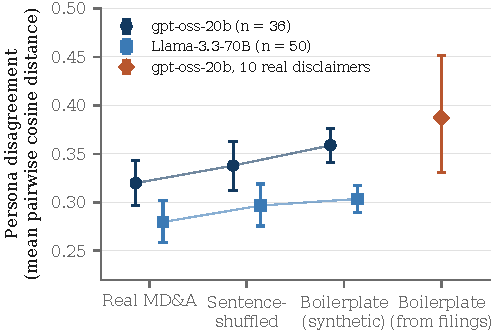
\includegraphics[width=\columnwidth]{figures/fig_r9_placebo.pdf}
  \caption{Content placebo. Mean persona disagreement with 95\% bootstrap CIs on real
  MD\&A windows, the same windows with sentences shuffled, and forward-looking-statement
  boilerplate. A valid complexity measure should fall on boilerplate. It rises, on both
  model families. The rightmost point uses \BpN{} distinct disclaimers taken from the
  sample's own filings and compares to all \BpRealN{} real windows.}
  \label{fig:placebo}
\end{figure}

\emph{Placebo.} On a stratified subset of \PlacN{} MD\&A windows we compared real text
with two degraded versions: sentences shuffled within the window, which destroys the
argument and keeps the vocabulary, and roughly 1,200 words of safe-harbor boilerplate,
which is real filing language with no firm-specific content. A measure of interpretive
complexity should fall on both. Shuffling is undetectable (\PlacDiffShuffled{}
[\PlacDiffShuffledLo, \PlacDiffShuffledHi]). Boilerplate scores \emph{higher}:
\PlacBoilerplate{} against \PlacReal{} for the real text (Figure~\ref{fig:placebo}).
The ordering real $<$ shuffled $<$ boilerplate replicates on
\XmModel{} at \texttt{bf16}, pinned to a single provider, on \XmN{} windows, with the
boilerplate contrast again clearing zero (\XmDiffBoil{} [\XmDiffBoilLo,
\XmDiffBoilHi]). Because a single synthetic passage cannot separate ``boilerplate
raises disagreement'' from ``this passage is odd,'' we also scored \BpN{} distinct
disclaimers harvested from the sample's filings. They average \BpMean{}
[\BpLo, \BpHi] against \BpRealMean{} for real MD\&A, with wide spread across passages
(SD \BpSD, range \BpMin{} to \BpMax). Content-free filing prose raises disagreement on
average; it does not do so uniformly.

\emph{What it responds to instead.} Across all scored windows, disagreement falls as
the share of numeric tokens rises ($\rho=\NumDensityRho$, $p\NumDensityP$), while word
count barely matters ($\rho=\InfWordCountRho$). It is higher in Risk Factors
(\DisagRisk) than MD\&A (\DisagMDA), higher at the start of a section, where overview
language sits ($\rho=\PosRho$ with position), and higher in windows that mention
litigation (\TopicLit) or guidance (\TopicGuid) than in windows about accounting
(\TopicAcct). The extreme windows show the mechanism in the text. The lowest-scoring
window in the sample (\CaseLowDisag) is a large technology firm's MD\&A opening dense
with growth figures, and all three personas cite the same percentages. The highest
large-cap window (\CaseHighDisag, numeric density \CaseHighDensity) is a bulleted list
of generic risk drivers; the value persona sees a durable moat, the language persona
sees hedged uncertainty, and the fundamentals persona writes that the excerpt ``offers
no quantitative evidence.'' Given nothing concrete, each lens fills the gap with its own
prior. The prompts make this likely by design: the language persona is explicitly asked
to assess vagueness, so vague text pushes it toward a different topic than the other
two.

\begin{figure*}[t]
  \centering
  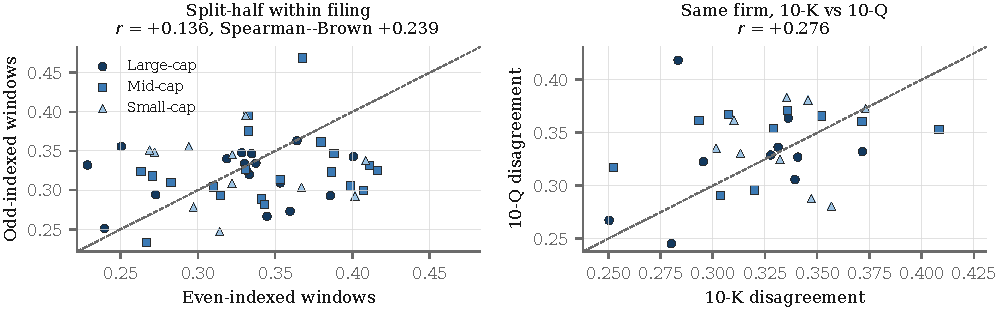
\includegraphics[width=0.78\textwidth]{figures/fig3_validity.pdf}
  \caption{Reliability of the filing-level measure. Left: odd- against even-indexed
  windows of the same filing ($n=\SplitHalfN$ filings with at least four windows).
  Right: a firm's 10-K against its 10-Q ($n=\TestRetestN$ firms).}
  \label{fig:reliability}
\end{figure*}

\emph{Reliability.} Odd and even windows of the same filing correlate at
$r=\SplitHalfR$, a Spearman--Brown reliability of \SplitHalfSB{} for the full filing
mean; a firm's 10-K and 10-Q correlate at $r=\TestRetestR$ (Figure~\ref{fig:reliability}).
\VarWithinFilingPct\% of window-level variance lies within filings, and the firm-level
intraclass correlation is \ICCFirm. Reaching a conventional reliability of 0.70 would
take about \RelWindowsSeventy{} windows, or \RelWordsSeventy{} words of MD\&A per
filing, far more than a typical filing has. More firms would not fix this. The secondary
numeric measure is more reliable (Spearman--Brown \SplitHalfSBNumeric), but, as the
next section shows, it runs against the hypothesis.

These results reconcile. The lenses do diverge; the divergence is driven by how much
concrete material a passage offers, which varies far more between windows of one filing
than between firms; so the filing mean is mostly noise, and what signal it has is
vagueness rather than difficulty.

% =====================================================================
\section{The Pre-Registered Size Test}
\label{sec:size}

\begin{table}[t]
  \caption{Pre-registered and exploratory size tests on firm-level MD\&A means
  ($n=\NFirms$ unless noted). Gradient is small minus large; the hypothesis predicts a
  positive gradient and a negative correlation with float.}
  \label{tab:size}
  \footnotesize\setlength{\tabcolsep}{4pt}
  \begin{tabular}{@{}lrrrrr@{}}
    \toprule
    Measure & Large & Mid & Small & Grad. & $p$ \\
    \midrule
    \multicolumn{6}{@{}l}{\emph{Secondary family, two-sided, Holm-adjusted $p$}} \\
    Numeric (score SD) & \SecNumLarge & \SecNumMid & \SecNumSmall & \SecNumGrad & \SecNumHolm \\
    Risk Factors ($n=\SecRiskFirms$) & & & & \SecRiskGrad & \SecRiskHolm \\
    Within-filing SD & & & & \SecSDGrad & \SecSDHolm \\
    \midrule
    \multicolumn{6}{@{}l}{\emph{Confirmatory, one-sided}} \\
    Embedding (C1) & \TierMeanLarge & \TierMeanMid & \TierMeanSmall & \PrimaryGradient & \PrimaryJTp \\
    \quad label permutation & & & & & \PrimaryPermP \\
    \quad excl.\ 1-filing firm ($n=\HaynN$) & & & & \HaynGrad & \HaynP \\
    \midrule
    \multicolumn{6}{@{}l}{\emph{Exploratory: Spearman $\rho$ with public float}} \\
    Embedding & \multicolumn{3}{r}{$\rho=\ContRho$ [\ContLo, \ContHi]} & & \ContP \\
    \bottomrule
  \end{tabular}
\end{table}

As the plan requires, the numeric measure comes first. Its firm-level means are
\SecNumLarge{} (large), \SecNumMid{} (mid) and \SecNumSmall{} (small): small-caps are
\emph{lowest}, the gradient is \SecNumGrad, and the two-sided test does not reject
($p=\SecNumP$, Holm \SecNumHolm). The pre-registered rule for retiring it as a length
proxy did not trigger ($\rho=\NumericLengthRho$ with MD\&A length, $p=\NumericLengthP$).

The primary embedding measure gives \TierMeanLarge, \TierMeanMid{} and \TierMeanSmall:
a gradient of \PrimaryGradient{} in the predicted direction but not monotone. The
confirmatory test does not reject ($J=\PrimaryJT$, $z=\PrimaryJTz$, $p=\PrimaryJTp$;
permutation $p=\PrimaryPermP$). Dropping the one firm with a single filing, a
sensitivity specified in the plan, gives $p=\HaynP$. Risk Factors, where one might
expect divergence to live, is flat to negative (\SecRiskGrad), as is within-filing
dispersion (\SecSDGrad). Under the plan's definition this is a null on all three
grounds: the test is not significant, the means are not monotone, and the window-count
gate below fails.

\begin{figure}[t]
  \centering
  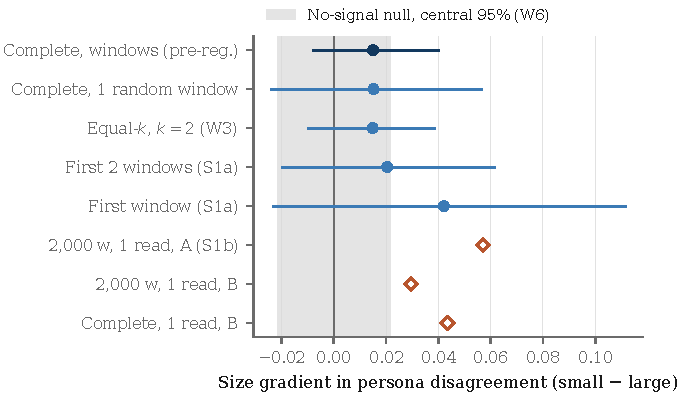
\includegraphics[width=\columnwidth]{figures/fig_r9_gradients.pdf}
  \caption{The size gradient under each scoring variant, with 95\% intervals where
  defined (bootstrap, or the 2.5th to 97.5th percentile of resamples). The grey band is
  the central 95\% of gradients produced by the pre-registered estimator when window
  values are reassigned at random, holding each filing's real window count fixed (W6).
  Open diamonds are single-read arms from Table~\ref{tab:harness}.}
  \label{fig:gradients}
\end{figure}

\textbf{Window-count artifacts.} Window count rises with tier ($\rho=\WOneRho$,
$p=\WOneP$): a large-cap MD\&A averages more windows. Averaging more windows reduces the
variance of a filing mean but not its expected value, so the channels that could bias
tier means are composition (a two-window MD\&A is half section opening) and window size
(tail merges produce windows of \WinWordsMin{} to \WinWordsMax{} words). The pre-registered battery tests
both with no new model calls. Subsampling exactly $k=2$ windows per filing keeps the
gradient's sign in \WThreeShare{} of 2,000 draws against a pre-declared threshold of
0.90, so the gate fails. A window-level mixed model with firm random intercepts gives a
small-versus-large coefficient of \WFiveSmallCoef{} [\WFiveSmallCIlo, \WFiveSmallCIhi];
the nested firm/filing specification did not converge and is reported as such. A coarsened-exact-matching estimate within window-count bins (\WTwoCEM), position
controls (first two windows: \WFourFirstTwo; dropping each section's opening window:
\WFourExclFirst) and exact-size windows only (\WSevenExact) keep the sign, none comes
close to significance, and one of the two bins that contain all three tiers reverses
it. Reassigning window values at random while holding real window counts
fixed produces a null centred on zero with standard deviation \WSixNullSD; the observed
gradient sits at its \WSixPercentile{}th percentile ($p=\WSixP$). Window counts, in other
words, add noise rather than manufacturing a gradient, and the observed gradient is
within the range that noise alone produces (Figure~\ref{fig:gradients}).

\textbf{Is the size variable too coarse?} Three tiers discard most of the variation in
size, which is the first objection to a null. We retrieved each firm's own reported
public float, which spans \ContFloatMinM{} million to \ContFloatMaxT{} trillion dollars
and orders the tiers almost perfectly ($\rho=\ContTierRho$). Against continuous float
the primary measure runs in the predicted direction, $\rho=\ContRho$ [\ContLo,
\ContHi], $p=\ContP$; the numeric measure runs the other way ($\rho=\ContNumRho$). The
null is not an artifact of binning. A modest negative relation with size cannot be
ruled out at $n=\NFirms$, but given Section~\ref{sec:validity} it would be a relation
between size and vague prose, not between size and interpretive difficulty.

% =====================================================================
\section{Discussion: Lessons for LLM Measurement Harnesses}
\label{sec:discussion}

The measure failed, and we think the way it failed generalizes. Disagreement among
prompted views of one text is an attractive quantity because it requires no labels. Our
results suggest it has a default reading that is not the intended one: when a passage
gives the model little to anchor on, differently-prompted outputs drift toward their
own priors and apart from each other. That is useful to know for anyone using
ensemble disagreement as a signal of difficulty, risk or uncertainty in financial
text~\cite{kuhn2023semantic}. It is also invisible to the checks people usually run. A
noise floor, an encoder swap and a battery of discriminant correlations all came back
clean.

On the harness side, three practices would have changed what we believed at several
points in this project. Pinning one serving backend at one precision, and logging it
per call, made it possible to see that a significant contrast weakened on a second
provider. Treating a parse failure as a failure, rather than computing disagreement
from the two personas that did respond, removed a bias that was concentrated in large
and mid-cap windows (Appendix~\ref{app:deviations}). Decomposing a contrast before
interpreting it reversed our reading of the paper's original headline.

\textbf{A reporting checklist.} We suggest that papers deriving a firm-level measure
from LLM readings of filings report, at minimum: (1) the reading budget and the share
of each document it covers, broken out by the variable of interest; (2) the scoring
unit and the aggregation rule; (3) the serving backend, precision and routing policy;
(4) a content placebo with boilerplate and shuffled text; (5) the reliability of the
aggregated measure (split-half and an intraclass correlation) at the unit where the
hypothesis lives; and (6) every pre-specified test, including the ones that failed.
None of these needs new model calls beyond a small placebo subset.

% =====================================================================
\section{Limitations}

Thirty firms is a measure-validation sample, and three tiers stand in for point-in-time
size data we did not have; the float test addresses the second point only in part. One
model family produced the main results, and the cross-model check covers the placebo
only. The noise-floor subset was cut short by rate limiting at \NoiseN{} windows. The
persona prompts are a design choice, and a lens set that did not ask one persona to
judge vagueness might behave differently. The decomposition of the truncation contrast
relies on a single-read arm with its own size-correlated long-context bias and on a
second backend. Public float in the at-scale sample is self-reported XBRL and includes
implausible values at the bottom of the range; we use rank statistics for that reason.
We report no market outcome. The vagueness reading rests on the placebo, the
informativeness correlations and the case studies; we did not collect human judgments,
and a blinded comparison of high- and low-disagreement windows, asking raters separately
which is harder to interpret and which is less concrete, is the most direct next test.

% =====================================================================
\section{Conclusion}

Persona disagreement under a fixed model is real at the level of a single window,
stable across encoders, and unrelated to length and tone, and it still does not
measure interpretive complexity: it rises on boilerplate, falls with concrete figures,
and averages to noise at the filing level. Its pre-registered size test is null. Along
the way, the harness choices that are usually left out of methods sections, from the
reading budget to the scoring unit to the serving provider, each moved a result that
would otherwise have been reported. We would rather the field check these things
routinely than learn about them one retraction at a time.

% \begin{acks}
% TODO: acknowledgments, if any, once authorship is settled.
% \end{acks}

\bibliographystyle{ACM-Reference-Format}
\bibliography{refs_v2}

\appendix

\section{Persona Prompts}
\label{app:prompts}
All three personas receive the same window and the same output schema: \texttt{SCORE}
(integer 0--100, 50 neutral, with a calibration guide), \texttt{CONFIDENCE} (0--1),
\texttt{REASONING} (3--5 sentences citing the text) and \texttt{KEY\_FACTORS} (3--5
items). They differ only in framework. The \emph{value} persona weighs intrinsic value,
durable advantage, balance-sheet strength and free cash flow. The \emph{sentiment and
language} persona assesses how management communicates, including ``the specificity or
vagueness of strategic language.'' The \emph{fundamentals} persona weighs revenue and
margin trends, execution, and gaps between management claims and reported numbers.
Full prompt text is in \texttt{agents/prompts.py} at \url{https://github.com/aryanch09/interpretive-complexity-pilot}.

\section{Deviations from the Plan}
\label{app:deviations}
\begin{enumerate}
\item \textbf{Backend switched, then switched back} (before scoring, and before any
statistic was computed). The pinned provider was rate-limiting too heavily to finish;
the run moved to the only other \texttt{bf16} provider, which then degraded (slow
responses and empty completions). The 14 firms scored there were discarded, not merged,
and all \NFirms{} firms were re-scored on the original provider.
\item \textbf{Parse failures now count as failures} (mid-run, before any statistic).
The code had treated a persona that returned unparseable text as a success, keeping
the window with a two-score standard deviation and, where no rationale could be
extracted, a stand-in string for the embedding. That is imputation, which the plan
forbids. Twenty-five of the first 331 windows were affected, split 14 large / 11 mid /
0 small.
\item \textbf{Interpretation of the truncation contrast corrected} (after the number was
computed). The contrast was originally reported as truncation manufacturing a false
positive; the same-backend decomposition (Section~\ref{sec:harness}) shows it cannot be
attributed to coverage. The original figures are retained in Table~\ref{tab:harness}.
\end{enumerate}
Not deviations: the extraction fix, persistence of per-window rationales, and a score
parser correction were all declared in the plan before scoring.

\end{document}
